
% ==================================================
%	Theorie
% ==================================================

\section{Theorie}
\subsection{Die verlustfreie und reale Leitung}
Um die Eigenschaften einer verlustfreien Leitung zu modellieren kann das in
Abbildung~\ref{fig:verlust} dargestellte Ersatzschaltbild benutzt werden,
wobei $L$ eine
Spule und $C$ einen Kondensator darstellen. Um nun eine reale, verlustbehaftete
Leitung zu simulieren werden die Widerstände $R$ und $G$ gemäß
Abbildung~\ref{fig:verlust} in das Ersatzschaltbild integriert. Eine reale Leitung
wird nun durch den Kapazitätsbelag $C$, den Induktivitätsbelag $L$, den ohmschen
Belag $R$ und den Querleitfähigkeitsbelag $G$ charakterisiert. Die (komplexe)
Spannung $U(t,z)$ zur Zeit $t$ am Ort $z$ kann dann durch
\begin{equation}
U(t,z)=U_0 \e^{-\gamma z}\e^{\i\omega t} \label{eq:Spannung}
\end{equation}
beschrieben werden, wobei $\gamma=\alpha + \beta \i =\sqrt{(R+\i \omega L)(G+\i
\omega C)}$ die Ausbreitungskonsante mit dem Dämpfungsbelag $\alpha$ und dem
Phasenbelag $\beta$ ist und $\omega$ die Kreisfrequenz der angelegten Spannung mit
Amplitude $U_0$. Daraus
lässt sich der Wellenwiderstand $Z_0$ ableiten als das Verhältnis von
Spannungsamplitude zu Stromamplitude
\begin{equation}
Z_0:= \frac{U(\omega)}{I(\omega)} = \sqrt{\frac{R+\i \omega L}{G+\i \omega C}}
\label{eq:Wellenwiderstand} \quad ,
\end{equation}
hier für den Spezialfall, dass das Leitungskabel an jeder Stelle die gleichen
eigenschaften hat. Durch die Frequenzabhängigkeit von~\eqref{eq:Spannung} und
\eqref{eq:Wellenwiderstand} kommt es zur Dispersion und somit zur Verzerrung von
Signalen, die auf die Leitung gegeben werden.
\begin{figure}[htpb]
  \centering
  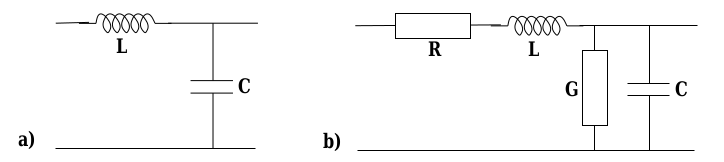
\includegraphics[scale=0.5]{bilder/schaltung.png}
  \caption{Ersatzschaltbild der verlustfreien (a) und verlustbehafteten (b)
    Leitung.\cite{AP}}
\label{fig:verlust}
\end{figure}

\subsection{Spannungsimpulse auf Leitungen}
Oft ist es nützlich, das Verhalten eines Spannungsimpulses auf einer Leitung zu
untersuchen. Hierzu werden neben $Z_0$ noch die Quellenimpedanz $Z_\text{g}$ und
die Lastimpedanz $Z_\text{L}$ benötigt. Ist $U_0$ die Spannung des eingehenden
Impulses, und $U_\text{r}$ die des am anderen Ende reflektierten, so gilt für die
Spannung $U_\text{L}$ an der Lastimpedanz
\begin{equation}
U_\text{L}=U_0+U_\text{r} \quad.
\end{equation}
Außerdem lässt sich der Reflexionsfaktor $\Gamma$ als
\begin{equation}
\Gamma := \frac{U_\text{r}}{U_0} =\frac{Z_\text{L}-Z_0}{Z_L + Z_0} =|\Gamma|e^{\i
\varphi_\Gamma} \label{eq:Gamma}
\end{equation}
definieren. Die Signalspannung in Ortsdarstellung lässt sich dann mit einer
Laplacetransformation $\mathfrak{L}$ aus der
Impulsdarstellung gemäß
\begin{equation}
U_\text{r}(t)=\mathfrak{L}^{-1}(U_\text{r}(p))=\mathfrak{L}^{-1}(\Gamma(p)U_\text{h}
(p))
\end{equation}
bestimmen, wobei $\Gamma$ der Reflexionsfaktor in Impulsdarstellung ist, und
$U_\text{r}(p)$ und $U_\text{h}(p)$ die Spannung des reflektierten bzw.\ hinlaufenden
Spannungspulses ist. Diese Rechnung entspricht der Näherung, dass die Leitung nahezu
verlustfrei ist.\\
Bei einer aus zwei Kabeln zusammengesetzten Leitung kommen zu $\Gamma_g$ und
$\Gamma_L$, den Reflexionsfaktoren am Anfang und Ende der Leitung noch die
Reflaxinosfaktoren am Kabelübergang $\Gamma_l$ und $\Gamma_r$ für von links und
rechts einlaufende Spannungsimpulse hinzu. Der Impulsfahrplan in
\ref{fig:Impusfahrplan} zeigt das Verhalten eines Spannungsimpulses entlang der
Leitung. Wieder wird angenommen, dass es keine Verluste gibt bzw.\ dass der
Transmissionsfaktor gleich $(1-\Gamma_i)$ für $i\in\{ g,L,l,r \}$. Aus den am
Leitungsanfang bei $0,2T,4T,6T$ gemessenen Spannungen $U_0,U_1,U_2,U_3$ lassen
sich anhand des Schaubilds folgende Gleichungen ablesen:
\begin{align}
  \Gamma_l&=\frac{U_1}{U_0} \\
  \Gamma_L&=\frac{U_3}{U_2}+\frac{U_2}{U_0(1-\Gamma_l)}\\
  \Gamma_r&=\frac{U_3}{U_2 \Gamma_L}
\end{align}
\begin{figure}[htpb]
  \centering
  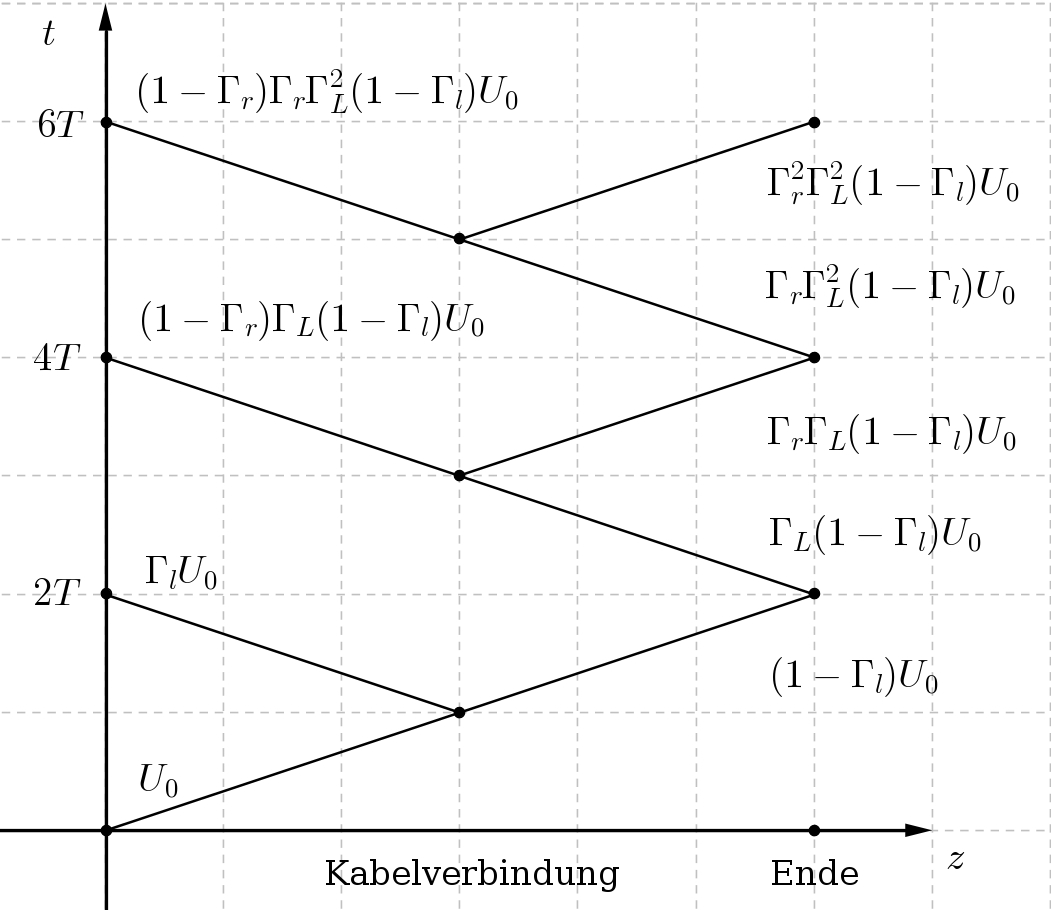
\includegraphics[scale=0.2]{bilder/fahrplan.jpg}
  \caption{Schematische Darstellung eines Spannungsimpulses auf einer Leitung.}
\label{fig:Impulsfahrplan}
\end{figure}

\subsection{Der Skin-Effekt bei Koaxialkabeln}
In diesem Verusuch werden Koaxialkabel verwendet. Diese bestehen aus einem inneren
Leiter als Kern. Dieser wird von einem Dielektrikum und dieses wiederum von einem
äußeren Leiter umgeben. Durch die magnetischen Felder innerhalb des Kabels werden
Wirbelströme induziert, welche den eigentlichen Wechselstrom an den äußeren Rand der
Leiter drängt, sodass der Leitungsquerschnitt verkleinert und somit der Widerstand
vergrößert wird. Aus diesem Grund wird der Widerstand $R$ eines Koaxialkabels bei
Kreisfrequenzen ab $100 \text{ kHz}$ durch ein $\sqrt{\omega}$-Gesetzt angemessen
beschrieben.
\subsection{Smith-Diagramme}
Smith-Diagramme sind ein Hilfsmittel, um zu einem gegebenen Lastwiderstand
$Z_\text{L}$ und Wellenwiderstand $Z_0$ den Reflexionsfaktor $\Gamma$ numerisch
zu ermitteln. Dazu wird~\eqref{eq:Gamma} mit $z_\text{L}:=Z_\text{L}/Z_0$
umgeschrieben zu
\begin{equation}
\Gamma = \frac{z_\text{L}-1}{z_\text{L}+1} \quad.
\end{equation}
Interpretiert man nun $\Gamma(z_\text{L})$ als komplexe Funktion ist dies eine
Möbiustransformation, sodass, da diese Abbildung konform ist, die Bilder der
Koordinatenachsen im Zielraum ebenfalls ein Koordinatessystem bilden. Um nun hieraus
einen Reflexionskoeffizienten zu bestimmen, muss lediglich $z_\text{L}$ in das
transformierte Koordinatensystem eingetragen werden. Dieser Punkt entspricht, wenn
er in Kartesischen Koordinaten abgelesen wird gerade $\Gamma(z_\text{L})$.

%fig
